\documentclass[10pt,conference,compsocconf]{../IEEEtran}

\usepackage{xltxtra}
\usepackage{tabularx}
\usepackage{booktabs}
\usepackage[caption=false]{subfig}
\usepackage[numbers,sort&compress]{natbib}
%\setmainfont{Times New Roman}

\begin{document}

\title{idock: A Multithreaded Virtual Screening Tool for Flexible Ligand Docking}

\author{\IEEEauthorblockN {Hongjian Li\IEEEauthorrefmark{1}, Kwong-Sak Leung\IEEEauthorrefmark{1} and Man-Hon Wong\IEEEauthorrefmark{1}
\IEEEauthorblockA {\IEEEauthorrefmark{1} Department of Computer Science and Engineering\\
Chinese University of Hong Kong\\
Shatin, New Territories, Hong Kong, P.R. China\\
Email: hjli@cse.cuhk.edu.hk}}}

\maketitle

\begin{table*}
\centering
\begin{tabular*}
{\linewidth}
{@{\extracolsep{\fill}}rrrr}
\toprule
& Total records & No. of native ligands & No. of decoys\\
\midrule
\multicolumn{4}{l}{\textbf{Raw csv files}}\\
set 1 & 138,621 & 176 & 138,445\\
set 2 & 130,791 & 167 & 130,624\\
\noalign{\smallskip\smallskip}
\multicolumn{4}{l}{\textbf{Case study 1}}\\
set 1 & 347 & 176 & 171\\
set 2 & 331 & 167 & 164\\
\noalign{\smallskip\smallskip}
\multicolumn{4}{l}{\textbf{Case study 2}}\\
set 1 & 3,473 & 1,760 & 1,713\\
set 2 & 3,310 & 1,670 & 1,640\\
\noalign{\smallskip\smallskip}
\multicolumn{4}{l}{\textbf{Case study 3}}\\
set 1 & 276,890 & 138,445 & 138,445\\
set 2 & 261,248 & 130,624 & 130,624\\
\bottomrule
\end{tabular*}
\caption{Number of native ligand conformations and decoys in set 1 and set 2 in raw csv files and case studies 1, 2 and 3.}
\label{tab:sets_stats}
\end{table*}

\begin{figure}
\centering
\begin{tabular}{cc}
\subfloat[active.]
{
  \label{subfig:l1_f50_set1_active}
  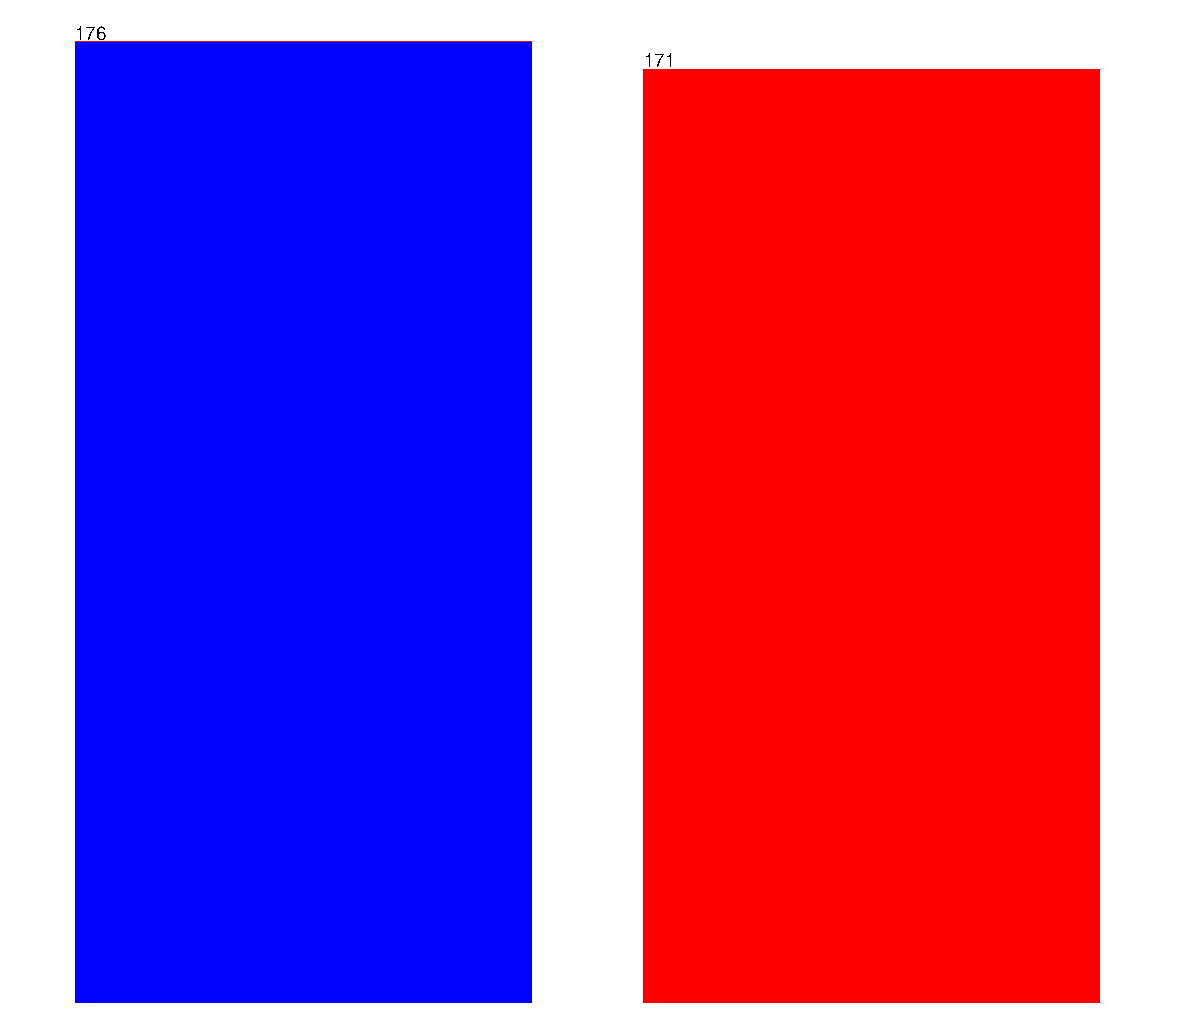
\includegraphics[width=0.46\linewidth]{Figures/l1_f50/set1/active.eps}
} &
\subfloat[gauss 1.]
{
  \label{subfig:l1_f50_set1_gauss1}
  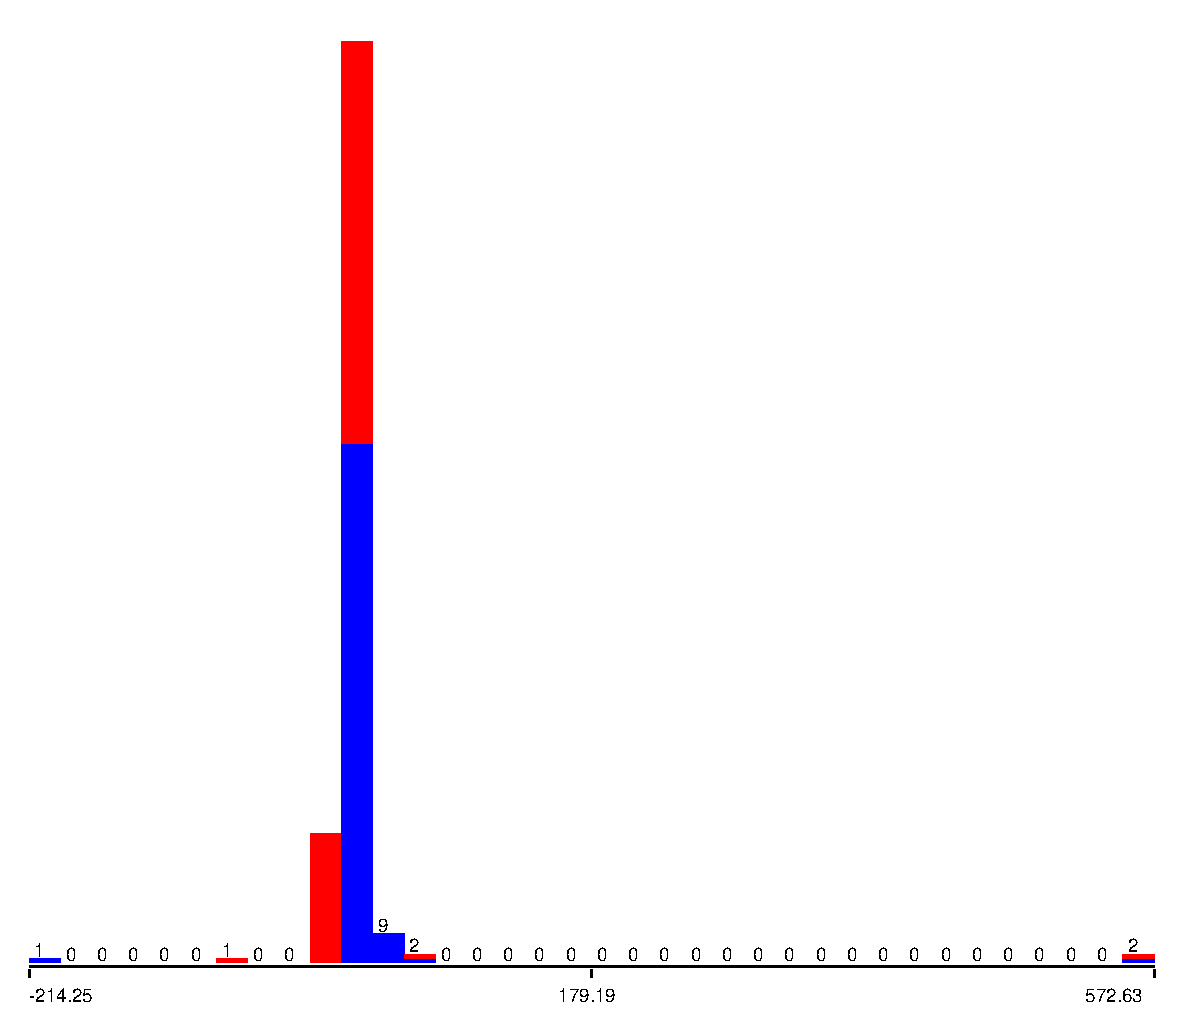
\includegraphics[width=0.46\linewidth]{Figures/l1_f50/set1/gauss1.eps}
} \\
\subfloat[gauss 2.]
{
  \label{subfig:l1_f50_set1_gauss2}
  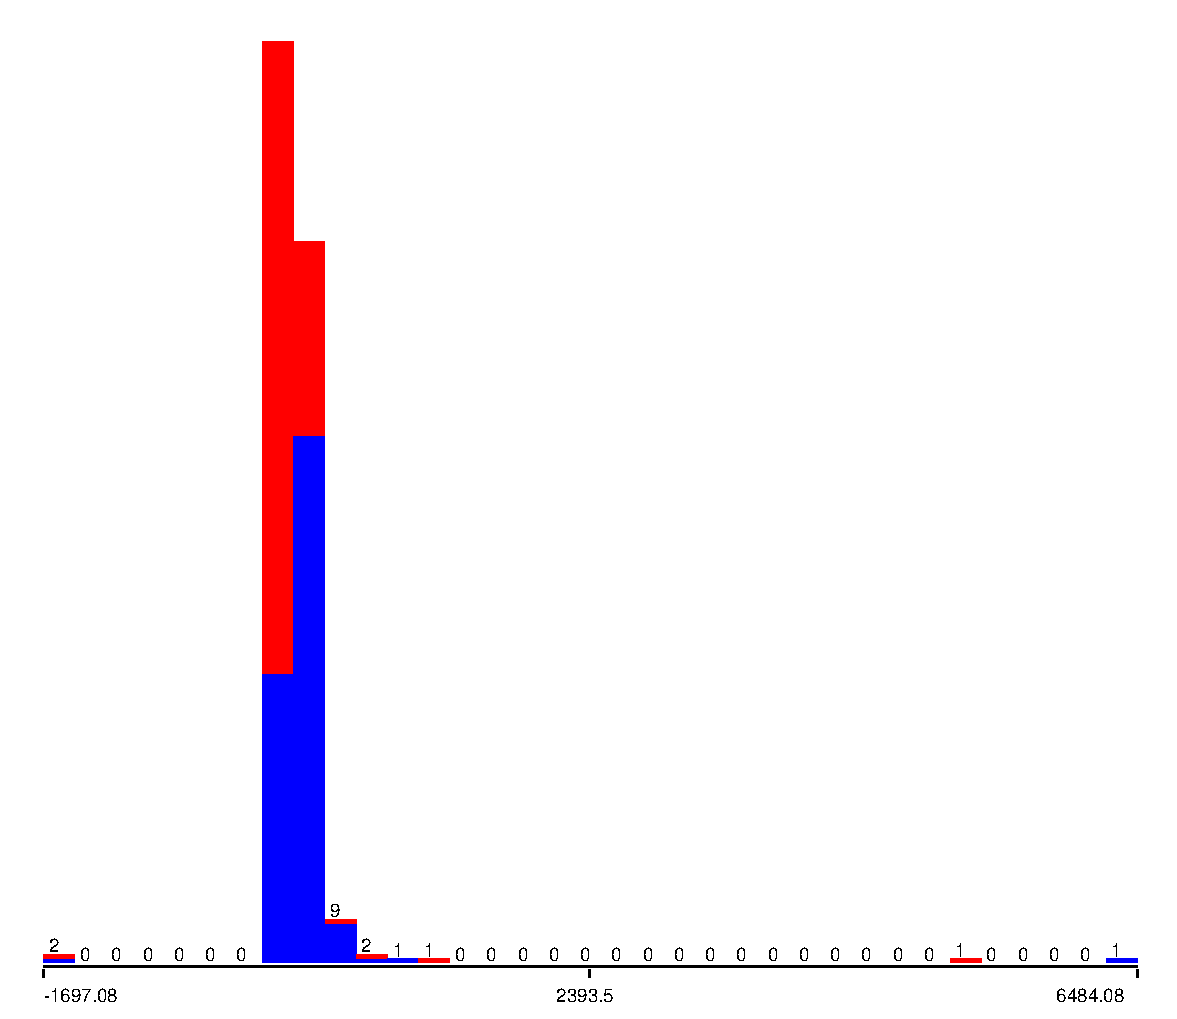
\includegraphics[width=0.46\linewidth]{Figures/l1_f50/set1/gauss2.eps}
} &
\subfloat[repulsion.]
{
  \label{subfig:l1_f50_set1_repulsion}
  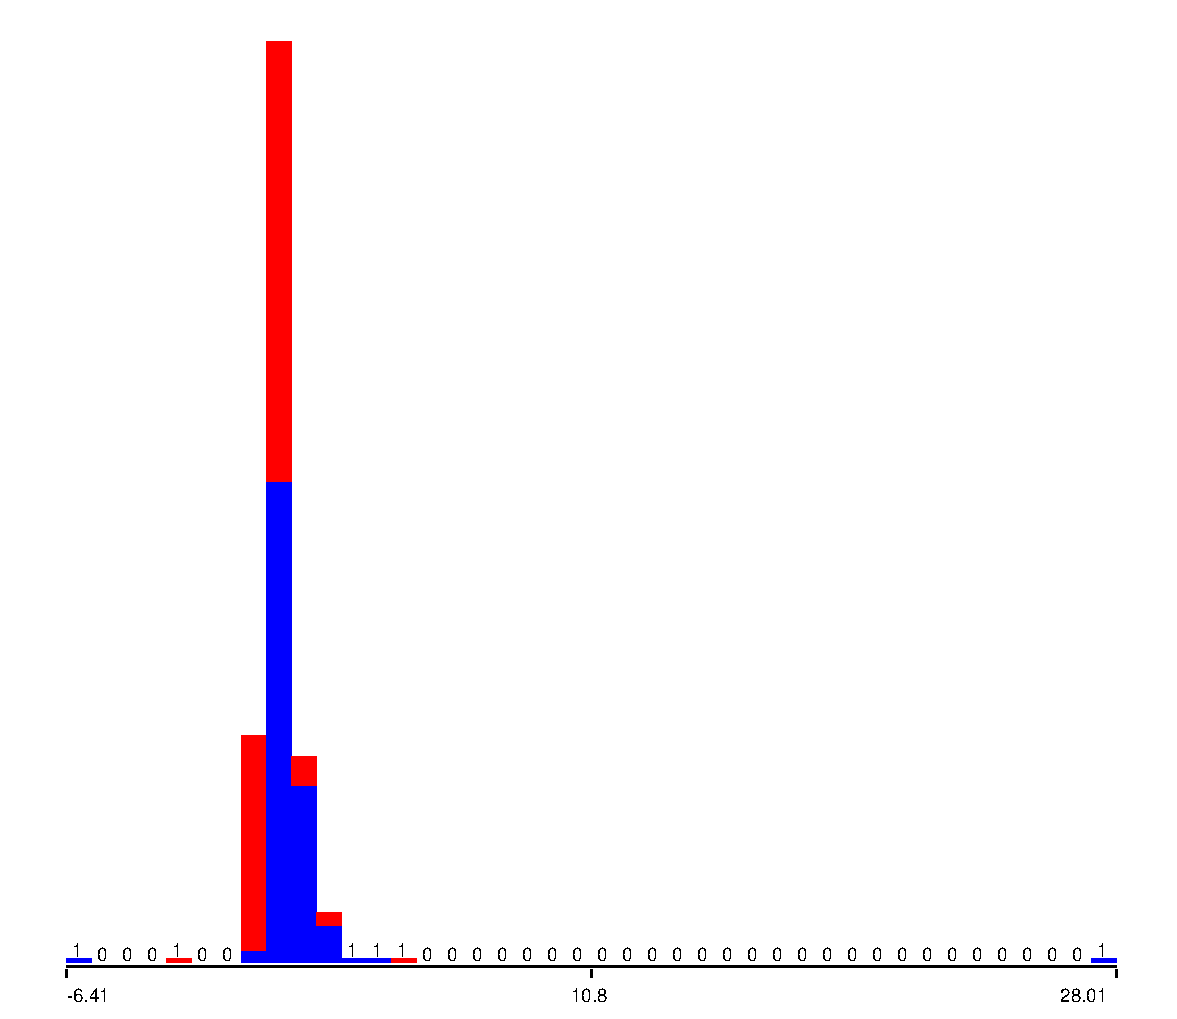
\includegraphics[width=0.46\linewidth]{Figures/l1_f50/set1/repulsion.eps}
} \\
\subfloat[hydrophobic interaction.]
{
  \label{subfig:l1_f50_set1_hydrophobic}
  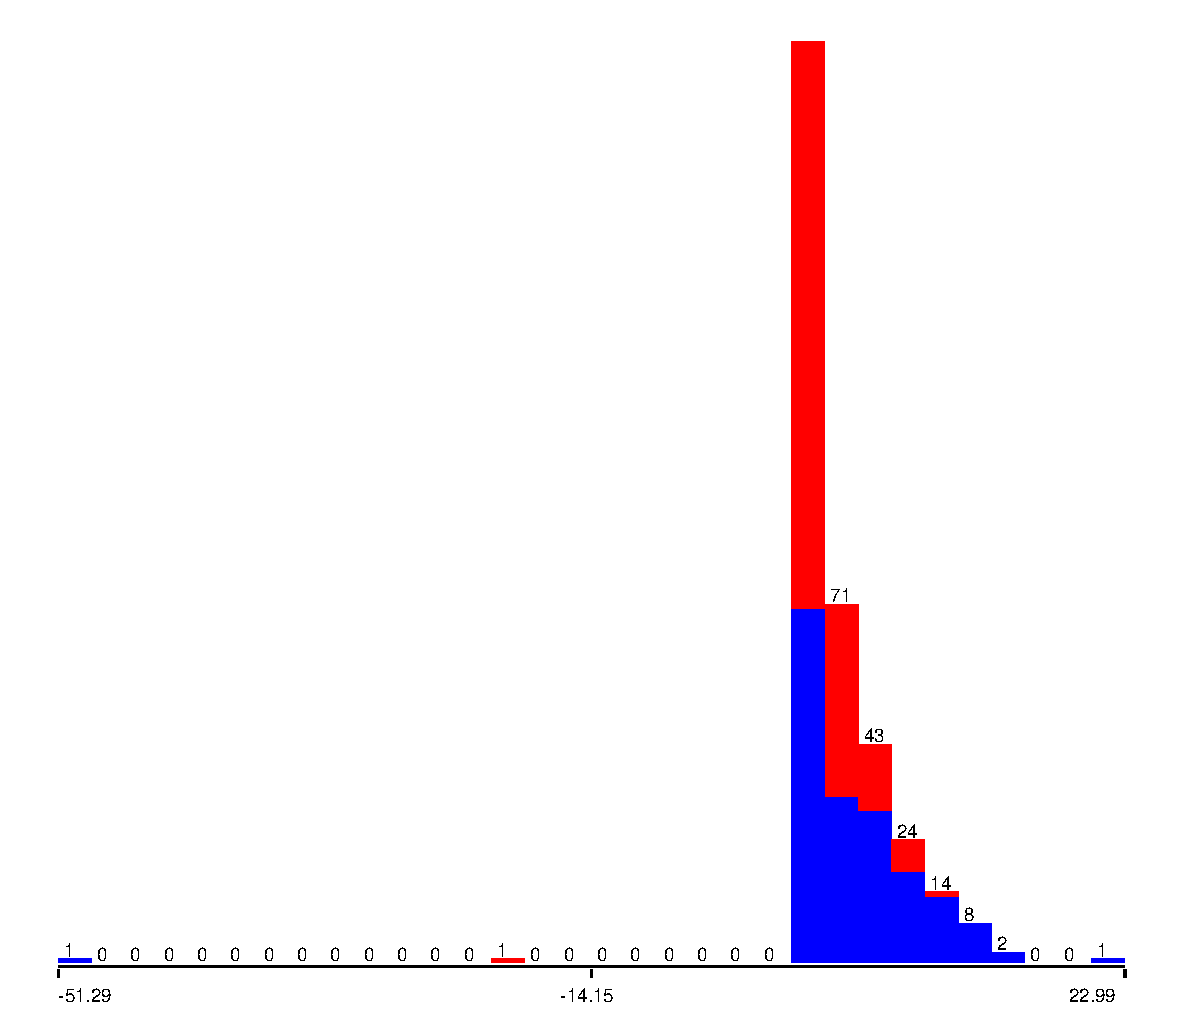
\includegraphics[width=0.46\linewidth]{Figures/l1_f50/set1/hydrophobic.eps}
} &
\subfloat[hydrogen bonding.]
{
  \label{subfig:l1_f50_set1_hydrogenbonding}
  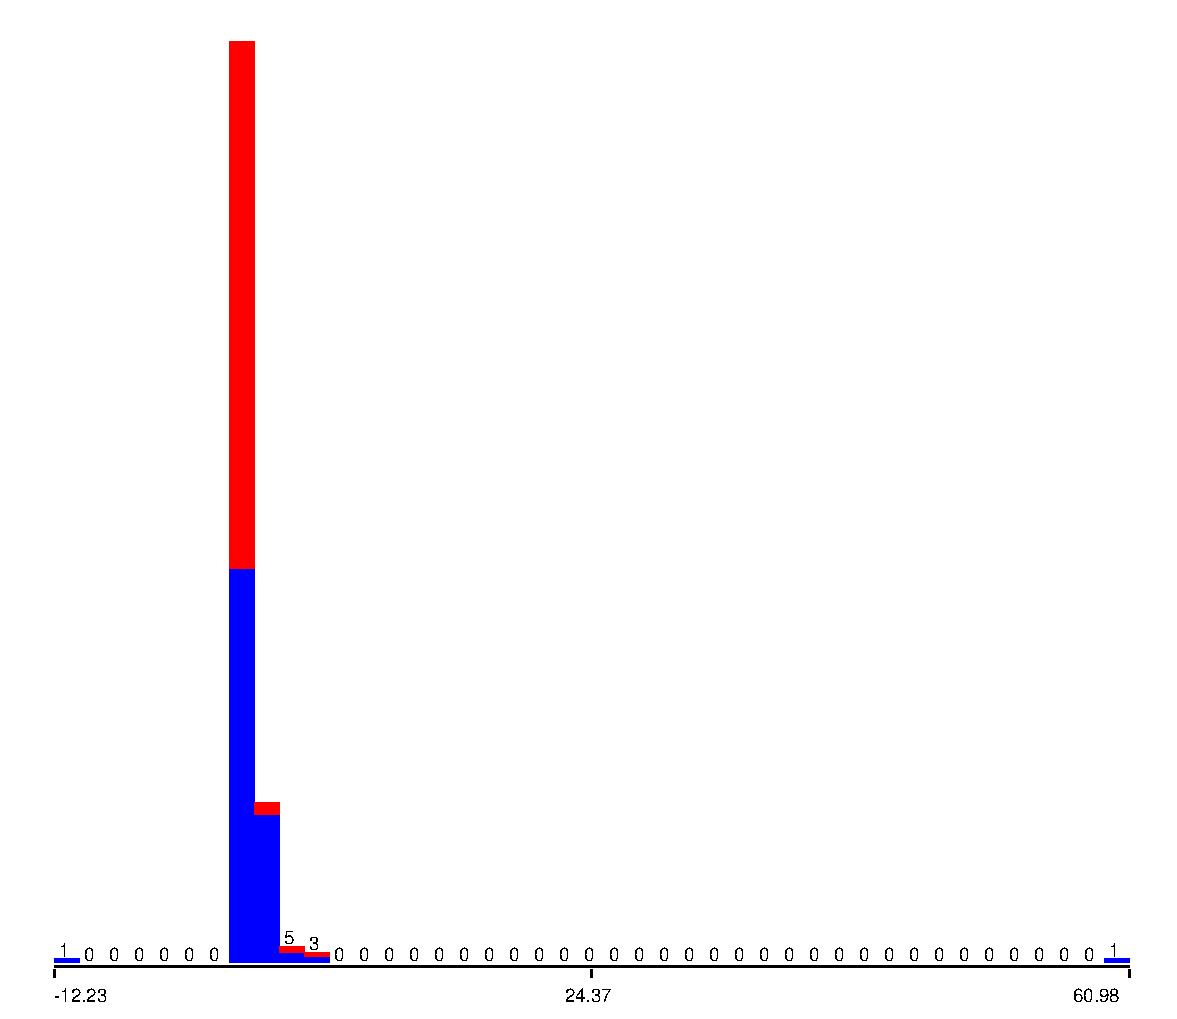
\includegraphics[width=0.46\linewidth]{Figures/l1_f50/set1/hydrogenbonding.eps}
} \\
\end{tabular}
\caption{Distributions of the 5 feature attributes and the binary class attribute of set 1 in case study 1. Class 1 is rendered in blue and class 0 is render in red.}
\label{fig:l1_f50_set1_dists}
\end{figure}

In \citeyear{970}, \Citeauthor{970} developed a program \citep{290,352}.
\citep{564,908,1281}
%\citep{773,712,377,983,916,304,1040,263,93,705,825,796,940,416,245,289,945,879,402,995,632,1001,357,356,1025,162,908,564,283,473,580,1008,210,1043,1042,878,297,365,518,539,540,537,105,872,793,515,990,824,993,640,548,461,690,675,260,598,978,314,599,937,912,848,1021,492,476,763,964,467,556,311,727,817,986,528,551,563,344,761,691,230,523,322,710,266,262,395,682,895,692,404,292,405,955,602,603,604,547,1005,637,481,332,307,421,355,321,281,927,318,979,764,650,709,725,989,469,804,787,615,233,427,331,889,738,441,930,857,960,999,171,1051,466,954,977,378,693,947,327,997,605,870,987,846,550,549,617,590,661,757,495,701,897,470,648,480,1018,373,721,741,583,890,438,694,1017,400,336,1032,1010,505,486,478,948,949,812,302,552,288,329,325,116,381,924,858,684,873,781,606,667,434,992,273,823,312,865,254,1013,967,272,256,287,487,491,726,291,360,982,534,941,944,462,856,613,502,407,337,353,841,663,962,1011,517,379,496,87,579,833,926,966,435,428,567,1038,784,770,282,533,532,557,743,276,315,88,299,359,1049,891,730,679,520,922,524,204,202,203,906,391,236,585,933,903,914,188,380,1023,301,956,704,115,896,424,317,414,819,797,483,565,608,482,538,792,280,309,686,931,932,1045,394,472,484,593,610,779,607,1039,794,724,961,774,270,805,452,996,894,90,1007,769,910,745,368,714,562,577,450,951,559,902,183,853,386,348,658,91,296,1037,277,303,1020,673,449,251,594,869,425,766,963,695,566,248,974,780,561,859,1024,971,290,750,970,1048,831,611,799,168,167,169,828,835,519,446,374,887,849,659,189,418,542,1035,760,729,795,867,881,330,938,1003,911,443,854,347,345,871,814,165,860,1002,436,772,762,464,366,300,278,349,735,939,791,811,578,584,408,493,844,861,976,597,596,920,506,601,664,925,991,512,535,1030,717,474,591,403,423,998,876,771,1016,362,786,444,782,959,410,1031,333,968,328,655,571,731,293,375,850,432,696,984,929,827,893,716,734,969,119,965,883,728,546,855,980,335,384,159,504,921,440,471,572,711,367,754,1041,429,308,209,498,923,560,905,525,909,439,840,943,672,981,261,574,320,163,697,454,880,242,739,1050,334,431,636,182,396,747,411,422,186,816,419,707,839,862,868,1026,626,733,788,785,830,676,268,269,543,123,1009,390,1006,455,363,588,522,677,813,884,129,181,609,600,975,1046,746,415,326,789,845,285,713,97,666,231,806,904,284,759,521,1028,1029,1000,586,680,815,350,433,581,453,776,832,685,843,448,808,503,744,698,748,740,286,426,722,723,958,900,838,442,1015,915,809,445,864,587,752,973,351,458,829,576,338,699,935,413,687,294,346,742,341,1012,187,279,393,211,1036,936,267,595,490,899,117,323,821,387,688,994,851,399,826,985,477,1027,185,456,736,120,479,886,901,888,485,382,1044,264,247,863,536,531,612,1019,401,972,389,305,950,801,529,530,342,118,343,573,569,526,175,934,681,582,385,810,96,952,802,370,371,928,618,820,275,274,671,570,751,383,1014,803,372,164,758,706,1034,837,575,463,875,885,917,913,919,749,907,376,516,352,866,720,475,489,669,643,614,398,988,775,652,437,392,777}

\bibliographystyle{unsrtnat}
\bibliography{../refworks}

\end{document}

